\documentclass[aps,prb,twocolumn,groupedaddress,amsmath,amssymb,
               superscriptaddress,nofootinbib,floatfix]{revtex4-2}

\usepackage{bm}
\usepackage{graphicx}
\usepackage{booktabs}
\usepackage{xcolor}
\usepackage{hyperref}
\usepackage{amsthm}
\usepackage{tikz}
\usetikzlibrary{arrows.meta,positioning}

\hypersetup{colorlinks=true,citecolor=blue!55!black,
            linkcolor=blue!55!black,urlcolor=blue!55!black,
            pdftitle={Rigorous Classification of a Massless Phase at the
                      Marginal Boundary of the Two-Dimensional Long-Range
                      XY Model}}
\theoremstyle{plain}
\newtheorem{theorem}{Theorem}
\newtheorem{lemma}{Lemma}
\newtheorem{corollary}{Corollary}
\theoremstyle{definition}
\newtheorem{assumption}{Assumption}
\newcommand{\BZ}{\mathrm{BZ}}
\newcommand{\dd}{\mathrm{d}}
\newcommand{\kmin}{k_{\min}}

\begin{document}

\title{Rigorous Classification of a Massless Phase at the Marginal Boundary
       of the Two-Dimensional Long-Range XY Model}

\author{Authors withheld for internal draft}
\affiliation{Affiliations to be finalized}
\date{\today}

\begin{abstract}
We rigorously classify a low-temperature regime of the marginal
two-dimensional long-range XY model as nonmagnetic and massless in the
precise sense of non-exponential two-point correlations.  For the
minimum-image, size-normalized $1/r^4$ interaction used in simulations, a
finite-volume infrared theorem proves, at every finite temperature,
\[
 \lim_{h\downarrow0}\limsup_{L\to\infty}m_{L,h}=0,
 \qquad
 \lim_{L\to\infty}\langle|\bm M_L|^2\rangle_{L,0}=0.
\]
The second limit follows from an exponential-tilt bridge between the
field-selected Bogoliubov bound and the symmetric zero-field observable.
Independently, at sufficiently low temperature, Ginibre comparison with the
nearest-neighbor XY model gives
\[
 \liminf_{L\to\infty}
 \langle\cos(\theta_0-\theta_x)\rangle_{L,0}
 \ge \frac{1}{8|x|}
\]
for every fixed $x\ne0$, excluding conventional exponential clustering.
Together these results establish the stated massless, nonmagnetic regime.
Explicit lattice estimates yield
$E_\infty(q)=(\pi c_\infty/2)|q|^2\log(1/|q|)+O(q^2)$.
A deterministic audit through $L=8192$ reproduces the exact logarithmic
coefficient below $10^{-6}$ relative error.  The resulting $\log\log L$
infrared divergence explains the severe finite-size ambiguity.  The exact
massless asymptotic law remains open: ordinary BKT behavior and logarithmic
quasi-long-range order are two leading possibilities, neither selected here.
\end{abstract}

\maketitle

\section{Introduction}

At a marginal long-range boundary, proving the absence of order settles only
half of the infrared problem.  A two-dimensional XY system can be
ferromagnetically ordered, nonmagnetic with conventional exponential
clustering, or nonmagnetic and massless.  The last category includes ordinary
BKT quasi-long-range order and potentially slower logarithmic correlations.
These alternatives are exceptionally difficult to separate numerically when
the infrared divergence is only doubly logarithmic.

Here we complete the phase-level classification that can be made rigorously
for the minimum-image, size-normalized $1/r^4$ XY model.  A direct
finite-volume theorem excludes ferromagnetic long-range order at every finite
temperature.  At sufficiently low temperature, an independent Ginibre
comparison supplies an algebraic two-point lower bound and excludes
conventional exponential clustering.  Their intersection is a positive
result: the low-temperature regime is nonmagnetic and massless in this
precise correlation sense.  The theorem does not determine its exact massless
decay law.

\begin{figure}[t]
\centering
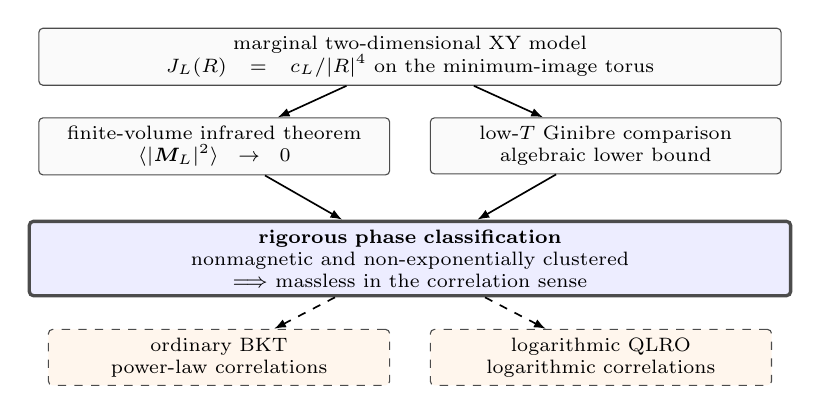
\begin{tikzpicture}[
  node distance=3.5mm and 3.5mm,
  every node/.style={font=\scriptsize,align=center},
  box/.style={draw=black!70,rounded corners=1.5pt,inner sep=3pt,
              fill=black!2},
  result/.style={box,very thick,fill=blue!7},
  endpoint/.style={box,dashed,fill=orange!7},
  proved/.style={-{Latex[length=1.5mm]},semithick},
  open/.style={-{Latex[length=1.5mm]},semithick,dashed}
]
\node[box,text width=.76\columnwidth] (model)
  {marginal two-dimensional XY model\\
   $J_L(R)=c_L/|R|^4$ on the minimum-image torus};
\node[box,text width=.35\columnwidth,below=4mm of model,
      xshift=-.205\columnwidth] (nolro)
  {finite-volume infrared theorem\\
   $\langle|\bm M_L|^2\rangle\to0$};
\node[box,text width=.35\columnwidth,below=4mm of model,
      xshift=.205\columnwidth] (lower)
  {low-$T$ Ginibre comparison\\
   algebraic lower bound};
\node[result,text width=.78\columnwidth,below=17mm of model] (massless)
  {\textbf{rigorous phase classification}\\
   nonmagnetic and non-exponentially clustered\\
   $\Longrightarrow$ massless in the correlation sense};
\node[endpoint,text width=.34\columnwidth,below=4mm of massless,
      xshift=-.20\columnwidth] (bkt)
  {ordinary BKT\\power-law correlations};
\node[endpoint,text width=.34\columnwidth,below=4mm of massless,
      xshift=.20\columnwidth] (log)
  {logarithmic QLRO\\logarithmic correlations};
\draw[proved] (model) -- (nolro);
\draw[proved] (model) -- (lower);
\draw[proved] (nolro) -- (massless);
\draw[proved] (lower) -- (massless);
\draw[open] (massless) -- (bkt);
\draw[open] (massless) -- (log);
\end{tikzpicture}
\caption{Logical classification of the marginal model.  Solid arrows are
proved implications.  Dashed arrows show two leading unresolved massless
scenarios; the present results neither select nor claim to exhaust them.}
\label{fig:phase-map}
\end{figure}

This conclusion reframes the apparent conflict with recent Monte Carlo
studies reporting a positive thermodynamic intercept at $\sigma=2$.  At the
marginal point the excitation kernel behaves as $q^2\log(1/q)$, so the
reciprocal infrared integral grows only as $\log\log L$.  Accessible sizes
can therefore remain close to an apparent magnetization plateau even though
the zero-field squared magnetization vanishes thermodynamically.  We keep the
analytic classification, the finite-size mechanism, and the numerical
convention audit logically separate.

The no-order ingredient is a general finite-volume infrared criterion.
Infrared bounds translate soft continuous-symmetry modes into restrictions
on spontaneous order; the Mermin--Wagner theorem supplies the canonical
short-range example \cite{MerminWagner1966}, while algebraic interactions can
be treated through the small-momentum excitation kernel
\cite{Bruno2001,Messager1984,Ioffe2002}.  A recurring technical mismatch is
that the bound is naturally formulated for a one-point magnetization selected
by a nonzero field, whereas finite simulations at zero field extrapolate
\begin{equation}
 \langle|\bm M_L|^2\rangle_{L,0}.
\label{eq:sim-observable}
\end{equation}
Global symmetry makes $\langle\bm M_L\rangle_{L,0}=0$ at every finite
$L$, but it does not make Eq.~\eqref{eq:sim-observable} vanish.

Recent Monte Carlo studies of the two-dimensional model
\begin{equation}
 J(r)\propto r^{-2-\sigma}
\end{equation}
reported a ferromagnetic phase up to and including $\sigma=2$
\cite{Xiao2025,Yao2025}.  At that endpoint the interaction is $1/r^4$ and
the kernel is
\begin{equation}
 E(q)\sim \rho_{\log}q^2\log(1/q).
\label{eq:marginal-intro}
\end{equation}
We separate the reusable theorem from the phase classification of this
particular model.  The
general result concerns any sequence of ferromagnetic XY torus couplings
whose Fourier kernels have a uniform limit with a divergent regulated
infrared integral.  Its new observable-level step is
\begin{equation}
\begin{gathered}
 \text{field-selected infrared bound}\\
 {}+\text{ exponential-tilt bridge}\\[-0.2em]
 \Longrightarrow
 \langle|\bm M_L|^2\rangle_{L,0}\longrightarrow0.
\end{gathered}
\label{eq:logical-chain}
\end{equation}
The minimum-image $1/r^4$ sequence is then proved to satisfy the abstract
hypotheses.  Numerical calculations serve only as an auditable convention
check; the theorem is analytic.

\section{General finite-volume criterion}

Fix an integer $d\ge1$.  For even $L$, let
$T_L=(\mathbb Z/L\mathbb Z)^d$ and $N=L^d$.  Consider
translation-invariant couplings
\begin{equation}
 J_L(R)=J_L(-R)\ge0,
 \qquad R\in T_L\setminus\{0\},
\label{eq:general-coupling}
\end{equation}
and the field-regulated Hamiltonian
\begin{equation}
 H_{L,h}
 =
 -\frac12\sum_{x\in T_L}\sum_{R\ne0}
 J_L(R)\cos(\theta_x-\theta_{x+R})
 -h\sum_x\cos\theta_x .
\label{eq:general-H}
\end{equation}
The pair factor includes self-inverse torus displacements.  At
$T=\beta^{-1}>0$, write $\langle\cdot\rangle_{L,h}$ for the Gibbs
expectation and define
\begin{equation}
 \bm M_L=\frac1N\sum_x(\cos\theta_x,\sin\theta_x),
 \qquad
 m_{L,h}=\langle M_L^{(1)}\rangle_{L,h}.
\label{eq:general-M}
\end{equation}

For torus momentum $q=2\pi n/L$, set
\begin{equation}
 E_L(q)=
 \sum_{R\ne0}J_L(R)[1-\cos(q\cdot R)].
\label{eq:general-kernel}
\end{equation}
Using fixed integer representatives for $R$, the same expression defines a
continuous periodic function on $\BZ=[-\pi,\pi]^d$.

\begin{assumption}[Uniform kernel limit]
\label{ass:uniform}
There is a continuous nonnegative periodic $E_\infty$ such that
\begin{equation}
 \|E_L-E_\infty\|_\infty\longrightarrow0.
\label{eq:uniform-assumption}
\end{equation}
\end{assumption}

\begin{assumption}[Infrared divergence]
\label{ass:infrared}
For
\begin{equation}
 I(h)=
 \int_\BZ\frac{\dd^dq}{(2\pi)^d}\,
 \frac1{h+E_\infty(q)},
\label{eq:Ih}
\end{equation}
one has
\begin{equation}
 \lim_{h\downarrow0}I(h)=\infty.
\label{eq:Ih-diverges}
\end{equation}
\end{assumption}

\begin{theorem}[Finite-volume infrared criterion]
\label{thm:general}
For the XY torus sequence \eqref{eq:general-H}, suppose
Eqs.~\eqref{eq:general-coupling}, \eqref{eq:uniform-assumption}, and
\eqref{eq:Ih-diverges} hold.  Then, for every $0<T<\infty$,
\begin{align}
 \boxed{\displaystyle
 \lim_{h\downarrow0}\limsup_{L\to\infty}m_{L,h}=0,}
\label{eq:general-field-result}\\
 \boxed{\displaystyle
 \lim_{L\to\infty}
 \langle|\bm M_L|^2\rangle_{L,0}=0.}
\label{eq:general-zero-result}
\end{align}
\end{theorem}

The theorem is dimension-independent but XY-specific.  It does not assert
an $O(n)$ extension without a separate rotation-generator proof.

\section{Proof of Theorem~\ref{thm:general}}

\subsection{Finite-volume field inequality}

\begin{lemma}[Classical Bogoliubov bound]
\label{lem:bog}
For every torus momentum $q$ and $h,T>0$,
\begin{equation}
 \boxed{\displaystyle
 1\ge
 Tm_{L,h}^2
 \frac1N\sum_q\frac1{h+E_L(q)}.}
\label{eq:bog}
\end{equation}
\end{lemma}

\begin{proof}
Introduce
\begin{equation}
 D_q=\sum_xe^{iq\cdot x}\frac{\partial}{\partial\theta_x},
 \qquad
 A_q=\sum_xe^{-iq\cdot x}\sin\theta_x .
\label{eq:D-A}
\end{equation}
Periodic integration by parts in the Gibbs measure gives
\begin{align}
 \langle D_qA_q\rangle
 &=\beta\langle A_qD_qH\rangle,
\label{eq:ibp-one}\\
 \langle D_{-q}D_qH\rangle
 &=\beta\langle|D_qH|^2\rangle.
\label{eq:ibp-two}
\end{align}
Cauchy--Schwarz therefore yields
\begin{equation}
 \langle|A_q|^2\rangle
 \langle D_{-q}D_qH\rangle
 \ge
 T|\langle D_qA_q\rangle|^2.
\label{eq:classical-bog}
\end{equation}
Direct differentiation gives
\begin{equation}
 D_qA_q=\sum_x\cos\theta_x,
 \qquad
 \langle D_qA_q\rangle=Nm_{L,h}.
\end{equation}
The registered pair convention in Eq.~\eqref{eq:general-H} gives exactly
\begin{multline}
 D_{-q}D_qH_{L,h}
 =h\sum_x\cos\theta_x\\
 +\sum_{x,R}J_L(R)[1-\cos(q\cdot R)]
 \cos(\theta_x-\theta_{x+R}).
\label{eq:second-derivative}
\end{multline}
Using $J_L\ge0$, $m_{L,h}\le1$, and $\cos u\le1$,
\begin{equation}
 \langle D_{-q}D_qH_{L,h}\rangle
 \le N[h+E_L(q)].
\label{eq:denominator-bound}
\end{equation}
Equations~\eqref{eq:classical-bog}--\eqref{eq:denominator-bound} imply
\begin{equation}
 \langle|A_q|^2\rangle
 \ge\frac{TNm_{L,h}^2}{h+E_L(q)}.
\end{equation}
Finally, discrete Parseval over the $N$ torus momenta gives
\begin{equation}
 \sum_q|A_q|^2
 =N\sum_x\sin^2\theta_x\le N^2.
\end{equation}
Summation over $q$ proves Eq.~\eqref{eq:bog}.
\end{proof}

\subsection{Fixed-field thermodynamic limit}

\begin{lemma}[Regulated limit]
\label{lem:regulated}
Under Assumption~\ref{ass:uniform}, for every fixed $h>0$,
\begin{equation}
 \limsup_{L\to\infty}m_{L,h}^2
 \le\frac1{TI(h)}.
\label{eq:regulated-bound}
\end{equation}
\end{lemma}

\begin{proof}
For nonnegative $x,y$,
\begin{equation}
 \left|\frac1{h+x}-\frac1{h+y}\right|
 \le\frac{|x-y|}{h^2}.
\end{equation}
Hence Eq.~\eqref{eq:uniform-assumption} implies uniform convergence of the
reciprocal kernels at fixed $h$.  The limiting reciprocal kernel is a
continuous periodic function, so the torus momentum average is a Riemann
sum:
\begin{equation}
 \frac1N\sum_q\frac1{h+E_L(q)}
 \longrightarrow I(h).
\label{eq:riemann}
\end{equation}
Take $\limsup$ in Eq.~\eqref{eq:bog}.  No existence assumption for
$\lim_Lm_{L,h}$ is required.
\end{proof}

\subsection{From a field to the zero-field second moment}

\begin{lemma}[Exponential-tilt inequality]
\label{lem:tilt}
Let $X\in[-1,1]$ have a distribution symmetric under $X\mapsto-X$.  For
$t\ge0$, define
\begin{equation}
 \mathbb E_t[f(X)]
 =
 \frac{\mathbb E[f(X)e^{tX}]}{\mathbb E[e^{tX}]}.
\end{equation}
Then
\begin{equation}
 \boxed{\mathbb E_tX\ge\tanh(t)\,\mathbb EX^2.}
\label{eq:tilt}
\end{equation}
\end{lemma}

\begin{proof}
Let $Q=|X|$.  Symmetry gives
\begin{equation}
 \mathbb E_tX
 =
 \frac{\mathbb E[Q\sinh(tQ)]}{\mathbb E[\cosh(tQ)]}
 =
 \mathbb E_w[Q\tanh(tQ)],
\label{eq:tilt-weight}
\end{equation}
where $\dd\mathbb P_w$ is proportional to
$\cosh(tQ)\dd\mathbb P$.  Both $Q\tanh(tQ)$ and $\cosh(tQ)$ are
nondecreasing.  For independent $Q,Q'$,
\begin{align}
 2\operatorname{Cov}(f(Q),w(Q))
 ={}&\mathbb E\bigl[(f(Q)-f(Q'))\nonumber\\
 &\qquad{}\times(w(Q)-w(Q'))\bigr]\ge0.
\end{align}
Thus the last expression in Eq.~\eqref{eq:tilt-weight} is at least
$\mathbb E[Q\tanh(tQ)]$.  Concavity of $\tanh$ and $\tanh(0)=0$ give
\begin{equation}
 \tanh(tQ)\ge Q\tanh(t),
 \qquad0\le Q\le1,
\end{equation}
which proves Eq.~\eqref{eq:tilt}.
\end{proof}

\begin{proof}[Proof of Theorem~\ref{thm:general}]
Lemma~\ref{lem:regulated} and Assumption~\ref{ass:infrared} give
\begin{equation}
 \limsup_{L\to\infty}m_{L,h}
 \le[TI(h)]^{-1/2}
 \xrightarrow[h\downarrow0]{}0,
\end{equation}
proving Eq.~\eqref{eq:general-field-result} with the physical order of
limits.

At $h=0$, global $O(2)$ invariance makes the law of
$X=M_L^{(1)}$ symmetric and exchanges the two spin components.  Therefore
\begin{equation}
 \langle X^2\rangle_{L,0}
 =
 \frac12\langle|\bm M_L|^2\rangle_{L,0}.
\label{eq:rotational-second-moment}
\end{equation}
The field changes the zero-field Gibbs weight by
\begin{equation}
 \exp\left(\beta h\sum_x\cos\theta_x\right)
 =\exp(\beta hL^dX).
\end{equation}
It is exactly the tilt of Lemma~\ref{lem:tilt} with
$t=\beta hL^d$.  Hence
\begin{equation}
 m_{L,h}
 \ge
 \frac12\tanh(\beta hL^d)
 \langle|\bm M_L|^2\rangle_{L,0}.
\label{eq:field-zero-bridge}
\end{equation}
Fix $h>0$ and take $L\to\infty$.  Since the hyperbolic tangent tends to one,
\begin{equation}
 \limsup_{L\to\infty}
 \langle|\bm M_L|^2\rangle_{L,0}
 \le
 2\limsup_{L\to\infty}m_{L,h}.
\end{equation}
Now let $h\downarrow0$.  The right-hand side vanishes by the field result.
The nonnegative left-hand side is independent of $h$, so it is zero.
\end{proof}

\section{Marginal two-dimensional corollary}

For even $L\ge8$, choose
\begin{equation}
 D_L=\{-L/2,-L/2+1,\ldots,L/2-1\}^2
\end{equation}
and define the exact minimum-image interaction
\begin{align}
 J_L(R)&=\frac{c_L}{|R|^4},
 &c_L&=\frac{\kappa}{S_L},\nonumber\\
 S_L&=\sum_{R\in D_L\setminus\{0\}}|R|^{-4},
 &\kappa&=4.
\label{eq:MI-coupling}
\end{align}
The fixed interaction is
\begin{align}
 S_\infty&=\sum_{R\in\mathbb Z^2\setminus\{0\}}|R|^{-4},
 &c_\infty&=\frac{\kappa}{S_\infty},\nonumber\\
 J_\infty(R)&=c_\infty|R|^{-4}.&&
\label{eq:fixed-coupling}
\end{align}
Extend $J_L$ by zero outside $D_L$ and call the extension $J_L^0$.

\begin{lemma}[Minimum-image kernel limit]
\label{lem:MI-limit}
The interaction and Fourier kernels obey
\begin{align}
 \|J_L^0-J_\infty\|_1
 &=2c_\infty(S_\infty-S_L)=O(L^{-2}),
\label{eq:l1-limit}\\
 \sup_{q\in[-\pi,\pi]^2}|E_L(q)-E_\infty(q)|
 &\le2\|J_L^0-J_\infty\|_1=O(L^{-2}).
\label{eq:kernel-limit}
\end{align}
\end{lemma}

\begin{proof}
Square-shell counting gives, for $r\ge2$,
\begin{equation}
 \sum_{|R|>r}|R|^{-4}
 \le8\sum_{n>\,r/\sqrt2}n^{-3}
 \le\frac{8\pi}{(r-1)^2}.
\label{eq:tail}
\end{equation}
Every point omitted from $D_L$ has $|R|>L/2-1$, so
$S_\infty-S_L=O(L^{-2})$.  Because
$c_LS_L=c_\infty S_\infty=\kappa$, the positive difference inside $D_L$
and the omitted tail outside it contribute equally to the $\ell^1$ norm,
giving Eq.~\eqref{eq:l1-limit}.  Equation~\eqref{eq:kernel-limit} follows
term by term from $|1-\cos(q\cdot R)|\le2$.
\end{proof}

\begin{lemma}[Marginal kernel]
\label{lem:marginal}
For $J_\infty(R)=A|R|^{-4}$ and $0<|q|\le1/2$,
\begin{equation}
 E_\infty(q)
 \le
 4A|q|^2
 \left[1+\log\frac2{|q|}+16\pi\right].
\label{eq:marginal-upper}
\end{equation}
Moreover,
\begin{equation}
 E_\infty(q)
 =
 \frac{\pi A}{2}|q|^2\log(1/|q|)
 +O(|q|^2).
\label{eq:marginal-exact}
\end{equation}
\end{lemma}

\begin{proof}
Split the sum at $|R|=|q|^{-1}$.  In the near region,
$1-\cos(q\cdot R)\le|q|^2|R|^2/2$ and
\begin{equation}
 \sum_{0<|R|\le M}|R|^{-2}
 \le8[1+\log(2M)].
\end{equation}
The far region is bounded by Eq.~\eqref{eq:tail} and
$1-\cos u\le2$.  This proves Eq.~\eqref{eq:marginal-upper}.

For the coefficient, lattice--continuum comparison gives
\begin{equation}
 \sum_{0<|R|\le M}\frac{R_iR_j}{|R|^4}
 =
 \pi\delta_{ij}\log M+O(1).
\label{eq:tensor-sum}
\end{equation}
The cell-comparison error is bounded because the gradient of
$x_ix_j/|x|^4$ is $O(|x|^{-3})$.  Taking $M=|q|^{-1}$ and expanding the
near part to second order, the Taylor remainder is
$O(q^4M^2)=O(q^2)$.  Contracting Eq.~\eqref{eq:tensor-sum} with
$Aq_iq_j/2$ yields Eq.~\eqref{eq:marginal-exact}; the far part is
$O(q^2)$.
\end{proof}

\begin{corollary}[No LRO at the marginal $1/r^4$ point]
\label{cor:marginal}
For the sequence \eqref{eq:MI-coupling} and every finite temperature,
\begin{equation}
 \boxed{\displaystyle
 \lim_{L\to\infty}
 \langle|\bm M_L|^2\rangle_{L,0}=0.}
\label{eq:marginal-result}
\end{equation}
\end{corollary}

\begin{proof}
Lemma~\ref{lem:MI-limit} verifies Assumption~\ref{ass:uniform}.  Write
Eq.~\eqref{eq:marginal-upper} as
$E_\infty(q)\le Cq^2\log(K/q)$.  On the annulus
$\sqrt h\le q\le q_0$,
\begin{equation}
 I(h)
 \ge
 \frac1{4\pi C}
 \log\left[
 \frac{\log(K/\sqrt h)}{\log(K/q_0)}
 \right]
 \xrightarrow[h\downarrow0]{}\infty.
\label{eq:loglog}
\end{equation}
Thus Assumption~\ref{ass:infrared} holds, and
Theorem~\ref{thm:general} applies.
\end{proof}

For the square lattice,
\begin{align}
 c_\infty&=\frac6{\pi^2G}
 =0.6637008046\ldots, \nonumber\\
 \rho_{\log}&=\frac{\pi c_\infty}{2}
 =1.0425387860\ldots .
\label{eq:rho-numeric}
\end{align}

\begin{figure*}[t]
 \centering
 
\includegraphics[width=0.94\textwidth]{paper/figures/kernel_audit.pdf}
 \caption{\label{fig:kernel}
 Deterministic audit of the exact minimum-image sequence through $L=8192$.
 (a) $E_L(\bm q)/|\bm q|^2$ follows the same logarithmic slope along four
 fixed momentum-index paths $\bm q=2\pi(n_x,n_y)/L$.
 (b) The intercept-free pair slope
 $\rho_{\rm eff}(L)=[Y_{2L}-Y_L]/\log2$ converges to
 $\rho_{\log}=\pi c_\infty/2$; the final relative discrepancies are below
 $9.1\times10^{-7}$.
 (c) $L^2$-scaled normalization corrections remain bounded, while the
 rigorous uniform-kernel comparison has the registered relative
 $O(1/\log L)$ scale at $k_{\min}$.  The calculation verifies conventions
 and numerical stability; it is not a premise of
 Corollary~\ref{cor:marginal}.}
\end{figure*}

\section{Relation to established theorems}

Bruno's theorem \cite{Bruno2001} is a quantum-spin magnetization result.  Its
Fourier criterion correctly includes the marginal $d=2$, $\alpha=4$ point,
but no formal $S\to\infty$ step is needed here:
Lemma~\ref{lem:bog} is directly classical.

Messager, Miracle-Sol{\'e}, and Ruiz (MMR) \cite{Messager1984} prove for
the fixed two-dimensional interaction a pointwise upper bound of the form
\begin{equation}
 |C(R)|
 \le B_2(\beta)[\log|R|]^{-\lambda_2(\beta)},
 \qquad \lambda_2(\beta)>0.
\label{eq:MMR}
\end{equation}
It is stronger pointwise information in its published thermodynamic-limit
scope, but it is an upper bound rather than an exact asymptotic law.

For the fixed $1/r^4$ interaction, define
$p(R)=J_\infty(R)/\kappa$.  Then
\begin{equation}
 1-\widehat p(q)=\frac{E_\infty(q)}{\kappa},
\end{equation}
and Eq.~\eqref{eq:marginal-upper} makes the associated walk recurrent.
Theorem 2 of Ioffe, Shlosman, and Velenik (ISV) \cite{Ioffe2002} therefore
implies that every fixed-model Gibbs state is $SO(2)$ invariant.

The scopes are complementary:
\begin{center}
\resizebox{\columnwidth}{!}{%
\begin{tabular}{lll}
\toprule
Route & Object & Conclusion\\
\midrule
Bruno & quantum fixed model & $m(T)=0$\\
MMR & classical fixed model & pointwise upper bound\\
ISV & classical fixed model & invariant Gibbs states\\
This work & XY torus sequence & zero-field $M_L^2\to0$\\
\bottomrule
\end{tabular}}
\end{center}

\section{Finite-size interpretation}

The same marginal kernel that proves Eq.~\eqref{eq:marginal-result} also
explains why the finite system looks ordered.  Consider, only as a scaling
family,
\begin{equation}
 C_L(Lx)=A[\ell+\phi(x)]^{-p},
 \qquad
 \ell=\log(L/L_0),\quad p>0.
\end{equation}
At large $\ell$,
\begin{equation}
 C_L(Lx)=A\ell^{-p}
 \left[1-\frac{p\phi(x)}{\ell}+O(\ell^{-2})\right].
\end{equation}
The constant term contributes at zero momentum but cancels at nonzero torus
momentum.  Consequently,
\begin{align}
 M^2(L)&\sim A\ell^{-p}\to0,\\
 M_{\kmin}^2(L)&\sim Bp\,\ell^{-p-1},\\
 \chi_{\kmin}&\sim BpL^2\ell^{-p-1},\\
 \left(\frac{\xi}{L}\right)^2
 &\sim\frac{\ell}{p}.
\label{eq:finite-signatures}
\end{align}
For small $p$, these relations look like
$\chi_{\kmin}\sim L^2/\log L$ and
$(\xi/L)^2\sim\log L$ while $M^2$ changes too slowly to reveal its zero
limit.

The Supplemental Material applies ordered, logarithmic, and BKT candidates
to the public summaries \cite{YaoData2025}, includes an exact Gaussian
known-zero control, profiles unavailable cross-observable covariance, and
quantifies synthetic recovery.  Those calculations explain finite-window
misidentification; none enters the theorem.

\begin{corollary}[Massless low-temperature regime]
\label{cor:massless}
Let $\beta_c^{\rm NN}$ be the critical inverse temperature of the
unit-coupling nearest-neighbor square-lattice XY model.  For every fixed
$x\ne0$,
\begin{equation}
 \beta\ge\frac{\beta_c^{\rm NN}}{c_\infty}
 \quad\Longrightarrow\quad
 \liminf_{L\to\infty}
 \left\langle
 \cos(\theta_0-\theta_x)
 \right\rangle_{L,0}
 \ge\frac{1}{8|x|}.
\label{eq:massless-lower}
\end{equation}
\end{corollary}

The proof embeds a fixed free nearest-neighbor box in the torus and uses
classical Ginibre monotonicity together with the low-temperature
nearest-neighbor theorem \cite{Ginibre1970,VanEngelenburgLis2023}; it is
given in the Supplemental Material.  The algebraic lower
bound~\eqref{eq:massless-lower} is incompatible with conventional
exponential clustering as $|x|\to\infty$.  Combined with
Corollary~\ref{cor:marginal}, it therefore proves a low-temperature regime
that is simultaneously nonmagnetic and massless.  Here \emph{massless} has
this precise correlation meaning: there is no finite-correlation-length
exponential upper bound.  It does not assert an exact correlation exponent.

\section{Massless phase and the infrared endpoint}

Theorem~\ref{thm:general} and Corollaries~\ref{cor:marginal}
and~\ref{cor:massless} exclude ferromagnetic LRO and a conventional
exponentially clustered low-temperature phase, but they do not select the
exact massless correlation law.
The rigorous classification is
\begin{equation}
 \boxed{\begin{gathered}
 \text{finite-temperature order: excluded;}\\
 \text{low-temperature massive endpoint: excluded;}\\
 \text{low-temperature massless regime: proved.}
 \end{gathered}}
\label{eq:phase-classification}
\end{equation}
Equation~\eqref{eq:MMR} is compatible with both a logarithmic decay and a
sufficiently slow power law.  Around a finite-temperature short-range BKT
fixed line, the long-range perturbation has linear eigenvalue
\begin{equation}
 \Delta_g=2-\sigma-\eta_{\rm sr}.
\end{equation}
At $\sigma=2$ and $\eta_{\rm sr}>0$, it is locally irrelevant
\cite{Giachetti2021}.  Coupled spin-wave--vortex work also supports
persistence of BKT behavior \cite{Walther2026}.  These are infrared
indications, not a global compact-field theorem.  Ordinary BKT behavior and
genuinely logarithmic quasi-long-range order are two leading unresolved
scenarios; the present results neither select nor claim to exhaust them.  A
proposed finite-momentum step response may help discriminate these scenarios,
but that is future work rather than evidence used in the present
classification.

\section{Conclusion}

We have rigorously classified the low-temperature marginal $1/r^4$ XY model
as nonmagnetic and massless in the correlation sense.  Two independent
ingredients are essential.  The finite-volume infrared theorem, completed by
an exponential-tilt bridge, gives
$\lim_{h\downarrow0}\limsup_{L\to\infty}m_{L,h}=0$ and
$\langle|\bm M_L|^2\rangle_{L,0}\to0$.  The low-temperature Ginibre
comparison gives an algebraic lower bound on the two-point function and rules
out conventional exponential clustering.  Neither statement alone yields
the classification; together they exclude both ferromagnetic order and a
conventional massive endpoint.

The exact minimum-image sequence satisfies the theorem through explicit
$O(L^{-2})$ interaction convergence and the marginal $q^2\log(1/q)$ kernel.
A multipath lattice audit reproduces the exact logarithmic coefficient and
verifies the simulation convention.  The associated $\log\log L$ divergence
supplies a mechanism for the exceptionally persistent finite-size plateau
without altering the thermodynamic conclusion.

What remains open is the asymptotic structure within the massless regime.
Ordinary BKT power-law behavior and genuinely logarithmic quasi-long-range
order are two leading scenarios, but the present theorem neither selects nor
claims to exhaust them.  Resolving that endpoint requires controlled
large-size information beyond the current public summaries.  The
theorem-level conflict is nevertheless settled: the low-temperature question
is no longer positive long-range order versus conventional massive
clustering, but the correlation law of an already established massless,
nonmagnetic regime.

\begin{acknowledgments}
Acknowledgments and funding information will be added after the author list
is finalized.
\end{acknowledgments}

\bibliography{paper/references}

\end{document}
